\documentclass[prb,12pt]{revtex4-2}

\usepackage{amsmath, amssymb,physics,amsfonts,amsthm}
\usepackage[most]{tcolorbox}
\usepackage{enumitem}
\usepackage{cancel}
\usepackage{booktabs}
\usepackage{polynom}
\usepackage{tabularx}
\usepackage{tikz}
\usepackage{hyperref}
\usepackage{enumitem}
\usepackage[normalem]{ulem}
\usepackage{transparent}
\usepackage{caption}
\usepackage{float}
\usepackage{multirow}
\newtheorem{Theorem}{Theorem}
\newtheorem{Proposition}{Theorem}
\newtheorem{Lemma}[Theorem]{Lemma}
\newtheorem{Corollary}[Theorem]{Corollary}
\newtheorem{Example}[Theorem]{Example}
\newtheorem{Remark}[Theorem]{Remark}
\theoremstyle{definition}
\newtheorem{Problem}{Problem}
\theoremstyle{definition}
\newtheorem{Definition}[Theorem]{Definition}
\newenvironment{parts}{\begin{enumerate}[label=(\alph*)]}{\end{enumerate}}
%tikz
\usetikzlibrary{patterns}
\usetikzlibrary{matrix}
%tcolorbox
\tcbset{breakable=true,toprule at break = 0mm,bottomrule at break = 0mm}
% definitions of number sets
\newcommand{\N}{\mathbb{N}}
\newcommand{\R}{\mathbb{R}}
\newcommand{\Z}{\mathbb{Z}}
\newcommand{\Q}{\mathbb{Q}}
\newcommand{\C}{\mathbb{C}}
\allowdisplaybreaks
\setlength{\parindent}{0cm}
\captionsetup[table]{name=Tabelle}

\begin{document}
\title{Fortgeschrittene Fehlerrechnung Übungsblatt 6}
	\author{Jun Wei Tan}
	\email{jun-wei.tan@stud-mail.uni-wuerzburg.de}
	\affiliation{Julius-Maximilians-Universit\"{a}t W\"{u}rzburg}
	\date{\today}
	\maketitle

\section{Bereingung der Untergrund}
Wir führen eine Messung durch und erhalten die folgenden Messwerte für die Zählereignisse eines befüllten Behälters und die Zählereignisse eines \emph{leeren} Behälters.

\setlength{\tabcolsep}{12pt}

\begin{center}
	\begin{tabular}{p{3cm}p{5cm}p{5cm}}
		\toprule
		\textbf{Winkel ($^\circ$)} & \textbf{Zählereignisse befülltes Behälters ($y_f$)} & \textbf{Zählereignisse leeres Behälters ($y_l$)}\\\midrule
		 155 & 184 & 5 \\\midrule
		135 & 134 & 4 \\\midrule
		120 & 99 & 4 \\\midrule
		100 & 49 & 1 \\\midrule
		90 & 53 & 3 \\\midrule
		75 & 55 & 1 \\\midrule
		65 & 70 & 4 \\\midrule
		55 & 81 & 9 \\\midrule
		40 & 130 & 8 \\\midrule
		20 & 216 & 7 \\\bottomrule
	\end{tabular}
\end{center}

Zur Bereinigung der Untergrund müssen wir die Zählereignisse bei einem leeren Behälter vom Zählereignisse bei einem befüllten Behälter abziehen. Es ist allerdings dabei zu beachten, dass die Anzahl der Teilchen in dieser Messung eine Hälfe die Anzahl beim Versuch mit einem befüllten Target, also wir müssen \emph{zweimal} $y_l$ vom $y_f$ abziehen. Wir bezeichnen die Anzahl der Ereignisse ohne Untergrund als $y$.
\begin{equation}
	y=y_f-2y_l
\end{equation}
Der Fehler kann nach Gauss fortgepflanzt werden:
\[\Delta y = \sqrt{(\Delta y_f)^2 + 4(\Delta y_l)^2}\]
	Wir nehmen an, dass die Anzahl der Ereignisse poissonverteilt ist. Daher ist der Fehler in $y_f$ $\Delta y_f=\sqrt{y_f}$ und analog f\"{u}r $\Delta y_l=\sqrt{y_l}$. Daraus ergibt sich
	\begin{equation}
		\Delta y = \sqrt{y_f+4 y_l}
	\end{equation}

\begin{center}
	\begin{tabular}{ccc}
	\toprule
	\textbf{Winkel ($^\circ$)} & $\cos\theta$ & \textbf{Zahlereignisse ohne Untergrund ($y$)}\\\midrule
		155 & -0.906308 & $174 \pm 14$ \\\midrule
135 & -0.707107 & $126 \pm 12$ \\\midrule
120 & -0.5 & $91 \pm 11$ \\\midrule
100 & -0.173648 & $47,0 \pm 7,3$ \\\midrule
90 & 0. & $47,0 \pm 8,1$ \\\midrule
75 & 0.258819 & $53,0 \pm 7,7$ \\\midrule
65 & 0.422618 & $62,0 \pm 9,3$ \\\midrule
55 & 0.573576 & $63 \pm 11$ \\\midrule
40 & 0.766044 & $114 \pm 13$ \\\midrule
20 & 0.939693 & $202 \pm 16$ \\\bottomrule
\end{tabular}
\end{center}

\section{Regression}
Wir suchen die Parameter $a_1,~a_2,~a_3\in \R$, sodass die folgende Funktion
\begin{equation}
	y(x)=a_1 P_0(x)+a_2 P_1(x)+a_3 P_2(x)
\end{equation}
die beste Anpassung an die Daten ist. Dabei sind $P_i,~i\in \{0,1,2\}$ die \emph{Legendre-Polynomen}
\begin{align*}
	P_0(x)&=1\\
	P_1(x)&=x\\
	P_2(x)&=\frac 12 (3x^2-1)
\end{align*}
Die Regressionskoeffizienten ergeben sich durch
\begin{align*}
	a_1&=\frac 1\Delta\begin{vmatrix}
		\sum y_i \frac{f_1(x_i)}{\sigma_i^2} & \sum \frac{f_1(x_i)f_2(x_i)}{\sigma_i^2} & \sum \frac{f_1(x_i)f_3(x_i)}{\sigma_i^2} \\
		\sum y_i \frac{f_2(x_i)}{\sigma_i^2} & \sum \frac{f_2(x_i)f_2(x_i)}{\sigma_i^2} & \sum \frac{f_2(x_i)f_3(x_i)}{\sigma_i^2} \\
		\sum y_i \frac{f_3(x_i)}{\sigma_i^2} & \sum \frac{f_3(x_i)f_2(x_i)}{\sigma_i^2} & \sum \frac{f_3(x_i)f_3(x_i)}{\sigma_i^2}
	\end{vmatrix}\\
	a_2&=\frac 1\Delta\begin{vmatrix}
	\sum \frac{f_1(x_i)f_1(x_i)}{\sigma_i^2} & \sum y_i \frac{f_1(x_i)}{\sigma_i^2} & \sum \frac{f_1(x_i)f_3(x_i)}{\sigma_i^2} \\
	\sum \frac{f_2(x_i)f_1(x_i)}{\sigma_i^2} & \sum y_i \frac{f_2(x_i)}{\sigma_i^2} & \sum \frac{f_2(x_i)f_3(x_i)}{\sigma_i^2} \\
	\sum \frac{f_3(x_i)f_1(x_i)}{\sigma_i^2} & \sum y_i \frac{f_3(x_i)}{\sigma_i^2} & \sum \frac{f_3(x_i)f_3(x_i)}{\sigma_i^2}
\end{vmatrix}\\
	a_3&=\frac 1\Delta\begin{vmatrix}
	\sum \frac{f_1(x_i)f_1(x_i)}{\sigma_i^2} & \sum \frac{f_1(x_i)f_2(x_i)}{\sigma_i^2} &  \sum y_i \frac{f_1(x_i)}{\sigma_i^2} \\
	\sum \frac{f_2(x_i)f_1(x_i)}{\sigma_i^2} & \sum \frac{f_2(x_i)f_2(x_i)}{\sigma_i^2} &  \sum y_i \frac{f_2(x_i)}{\sigma_i^2} \\
	\sum \frac{f_3(x_i)f_1(x_i)}{\sigma_i^2} & \sum \frac{f_3(x_i)f_2(x_i)}{\sigma_i^2} & \sum y_i \frac{f_3(x_i)}{\sigma_i^2}
\end{vmatrix}\\
	\Delta&=\begin{vmatrix}
		\sum \frac{f_1(x_i)f_1(x_i)}{\sigma_i^2} & \sum \frac{f_1(x_i)f_2(x_i)}{\sigma_i^2} & \sum \frac{f_1(x_i)f_3(x_i)}{\sigma_i^2} \\
		\sum \frac{f_2(x_i)f_1(x_i)}{\sigma_i^2} & \sum \frac{f_2(x_i)f_2(x_i)}{\sigma_i^2} & \sum \frac{f_2(x_i)f_3(x_i)}{\sigma_i^2} \\
		\sum \frac{f_3(x_i)f_1(x_i)}{\sigma_i^2} & \sum \frac{f_3(x_i)f_2(x_i)}{\sigma_i^2} & \sum \frac{f_3(x_i)f_3(x_i)}{\sigma_i^2}
	\end{vmatrix}
\end{align*}
Wir berechnen den Fehler analog wie Blatt 5. Daraus ergeben sich die Bestwerte
\begin{align*}
	a_1=&93,4\pm 3,4\\
	a_2=&-11,9\pm 6,6\\
	a_3=&104,3\pm 8,0
\end{align*}
\section{Güte der Anpassung}
Für eine qualitative Schätzung der Güte der Messung verwenden wir ein Residuenplot


Das Residuenplot zeigt, wie weit weg die Punkte von unserer Regressionskurve ist. Insgesamt ist die Streuung ordentlich und symmetrisch, also es gibt ungefähr die gleiche Anzahl von Punkte, die oberhalb und unterhalb der Nulllinie sind. Das heißt, dass die Streuung scheinbar zufällig verteilt ist. Die Werte mit Streuwinkel weniger als $60^\circ$ haben größer Fehler als die andere Werte. Das könnte an einem winkelabhängigen systematischen Fehler liegen, z.B. die Justierung des Messapparats. Außerdem ist es nur zu erwarten, dass 68,3\% der Messwerte innerhalb eines $\sigma$-Bandes liegen sollen, also einige Punkte mit größere Streuung ist auch zu erwarten. Insgesamt können wir die Anpassung als sinnvoll erachten. Für eine quantitative Schätzung der Güte könnten wir das $\chi^2$-Test verwenden. 

\begin{center}
	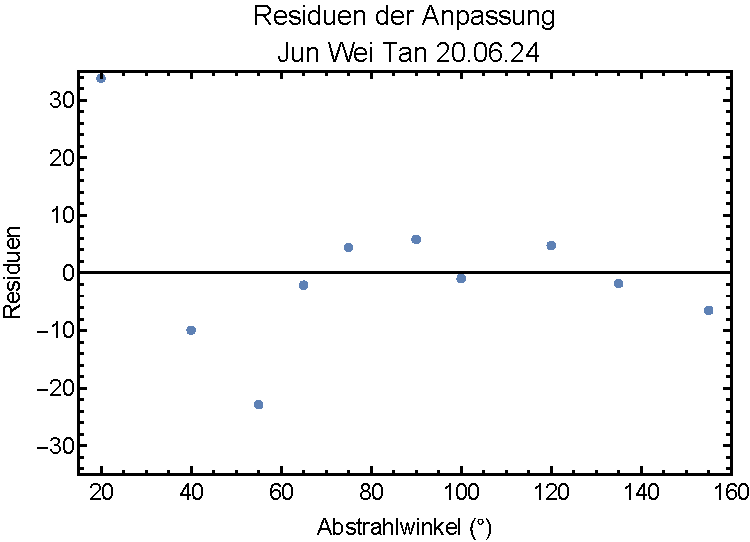
\includegraphics[width=0.8\textwidth]{plt2.pdf}
\end{center}
\begin{center}
	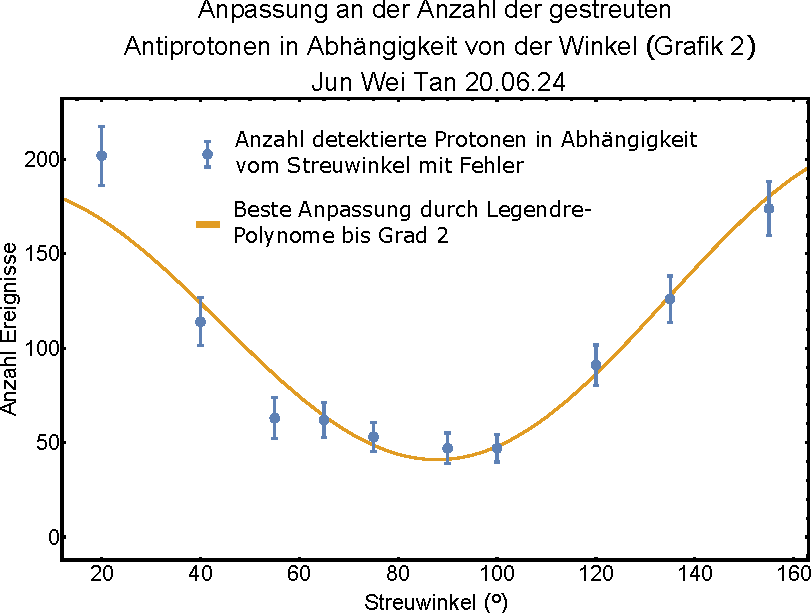
\includegraphics[width=0.8\textwidth]{fig.pdf}
\end{center}
\end{document}
